% !TeX spellcheck = cs_CZ
%{\tikzset{external/prefix={tikz/FYZII/}}
% \tikzset{external/figure name/.add={ch24_}{}}
%---------------------------------------------------------------------------------------------------
% file fey2ch24.tex
%---------------------------------------------------------------------------------------------------
%=========================== Kapitola Vlnovody =====================================================
\setchaptertoc
\chapter{Vlnovody}\label{fyz:IIchapXXIV}

  \section{Přenosové vedení}\label{fyz:IIchapXXIVsecI}
  \section{Obdélníkový vlnovod}\label{fyz:IIchapXXIVsecII}
  \section{Mezní frekvence}\label{fyz:IIchapXXIVsecIII}
  \section{Rychlost šíření vln ve vlnovodu}\label{fyz:IIchapXXIVsecIV}
  \section{Detekování vedených vln}\label{fyz:IIchapXXIVsecV}
  \section{Spojování vlnovodů}\label{fyz:IIchapXXIVsecVI}
  \section{Mody vlnovodů}\label{fyz:IIchapXXIVsecVII}
  \section{Jiný pohled na vlnovody}\label{fyz:IIchapXXIVsecVIII}
  \section{Příklady a cvičení}\label{fyz:IIchapXXIVsecIX}

    \begin{figure}[ht!] %\ref{fyz:fig559}
      \centering
      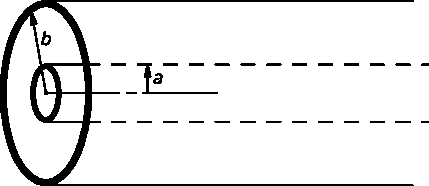
\includegraphics[width=0.7\linewidth]{fyz_fig559.pdf}
      \caption{
               (\cite[s.~707]{Feynman02})}
      \label{fyz:fig559}
    \end{figure}

    \begin{figure}[ht!] %\ref{fyz:fig560}
      \centering
      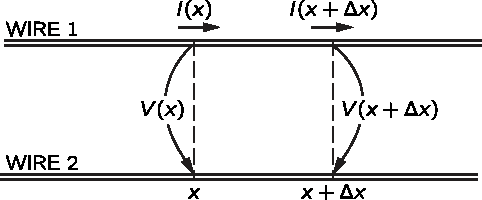
\includegraphics[width=0.7\linewidth]{fyz_fig560.pdf}
      \caption{
               (\cite[s.~707]{Feynman02})}
      \label{fyz:fig560}
    \end{figure}

    \begin{figure}[ht!] %\ref{fyz:fig561}
      \centering
      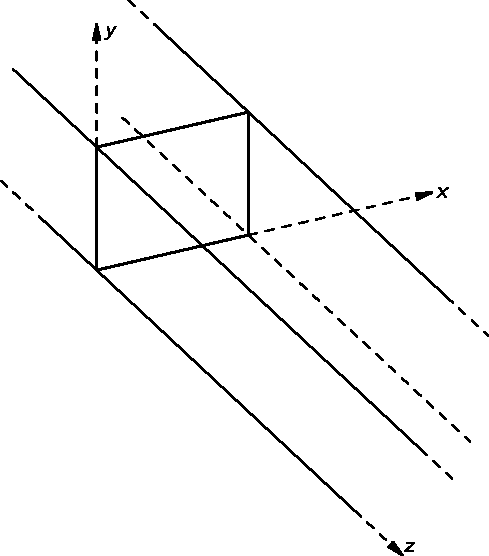
\includegraphics[width=0.7\linewidth]{fyz_fig561.pdf}
      \caption{
               (\cite[s.~707]{Feynman02})}
      \label{fyz:fig561}
    \end{figure}

    \begin{figure}[ht!] %\ref{fyz:fig562}
      \centering
      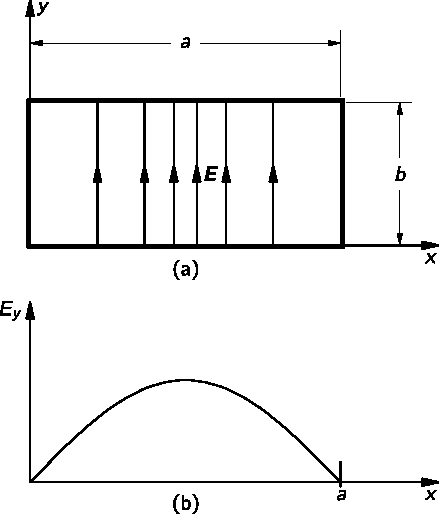
\includegraphics[width=0.7\linewidth]{fyz_fig562.pdf}
      \caption{
               (\cite[s.~707]{Feynman02})}
      \label{fyz:fig562}
    \end{figure}

    \begin{figure}[ht!] %\ref{fyz:fig563}
      \centering
      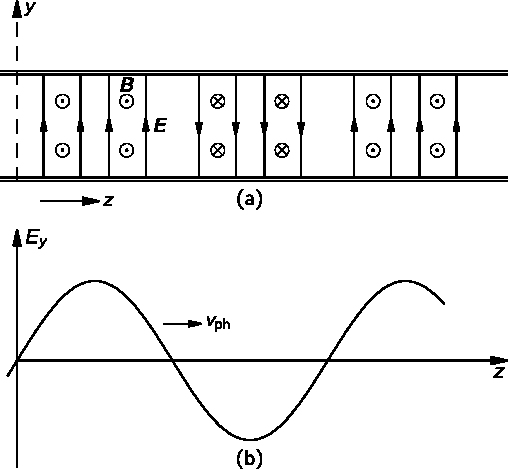
\includegraphics[width=0.7\linewidth]{fyz_fig563.pdf}
      \caption{
               (\cite[s.~707]{Feynman02})}
      \label{fyz:fig563}
    \end{figure}

    \begin{figure}[ht!] %\ref{fyz:fig564}
      \centering
      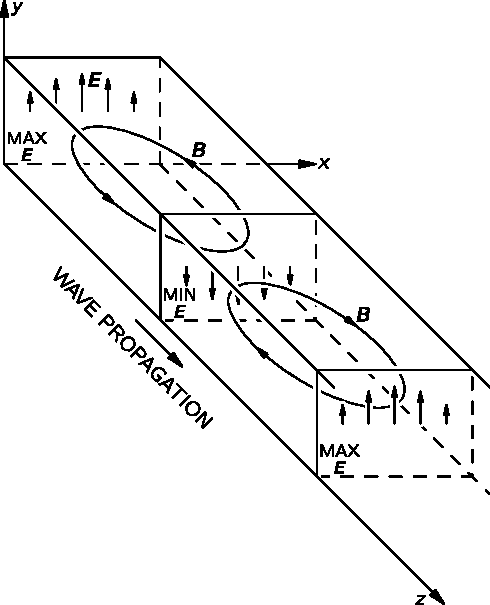
\includegraphics[width=0.7\linewidth]{fyz_fig564.pdf}
      \caption{
               (\cite[s.~707]{Feynman02})}
      \label{fyz:fig564}
    \end{figure}

    \begin{figure}[ht!] %\ref{fyz:fig565}
      \centering
      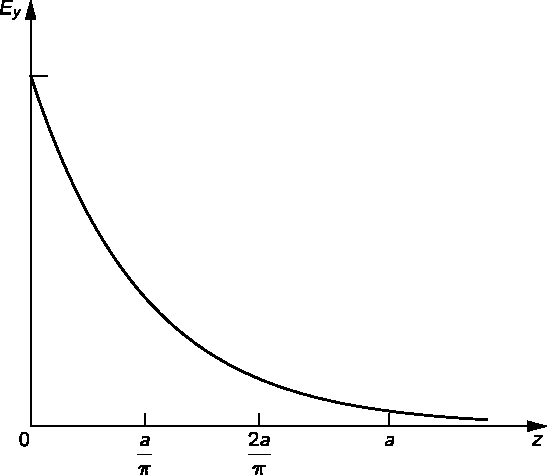
\includegraphics[width=0.7\linewidth]{fyz_fig565.pdf}
      \caption{
               (\cite[s.~707]{Feynman02})}
      \label{fyz:fig565}
    \end{figure}

    \begin{figure}[ht!] %\ref{fyz:fig566}
      \centering
      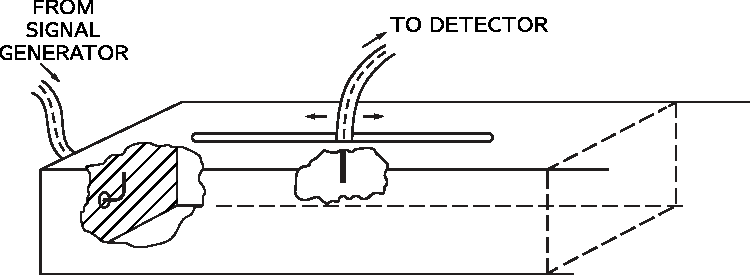
\includegraphics[width=0.7\linewidth]{fyz_fig566.pdf}
      \caption{
               (\cite[s.~707]{Feynman02})}
      \label{fyz:fig566}
    \end{figure}

    \begin{figure}[ht!] %\ref{fyz:fig567}
      \centering
      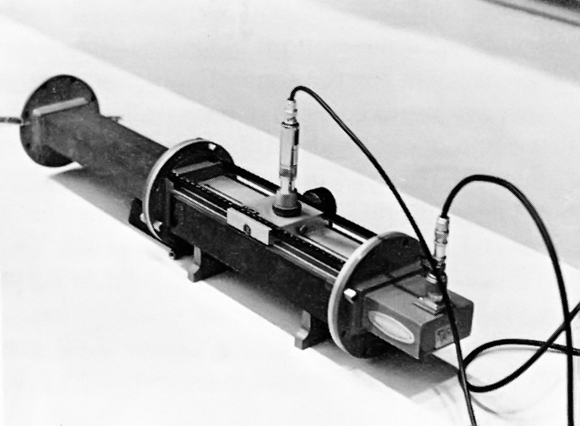
\includegraphics[width=0.7\linewidth]{fyz_fig567.jpg}
      \caption{
               (\cite[s.~707]{Feynman02})}
      \label{fyz:fig567}
    \end{figure}

    \begin{figure}[ht!] %\ref{fyz:fig568}
      \centering
      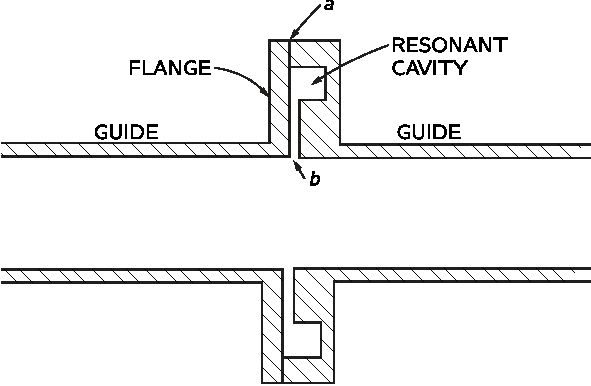
\includegraphics[width=0.7\linewidth]{fyz_fig568.pdf}
      \caption{
               (\cite[s.~707]{Feynman02})}
      \label{fyz:fig568}
    \end{figure}

    \begin{figure}[ht!] %\ref{fyz:fig569}
      \centering
      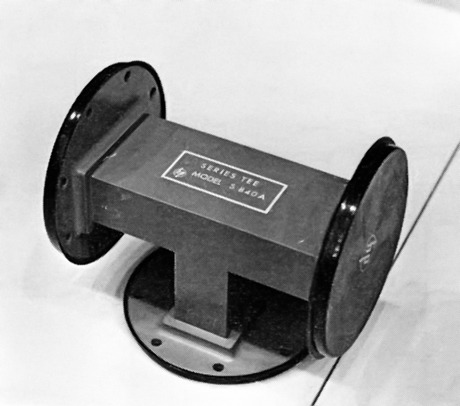
\includegraphics[width=0.7\linewidth]{fyz_fig569.jpg}
      \caption{
               (\cite[s.~707]{Feynman02})}
      \label{fyz:fig569}
    \end{figure}

    \begin{figure}[ht!] %\ref{fyz:fig570}
      \centering
      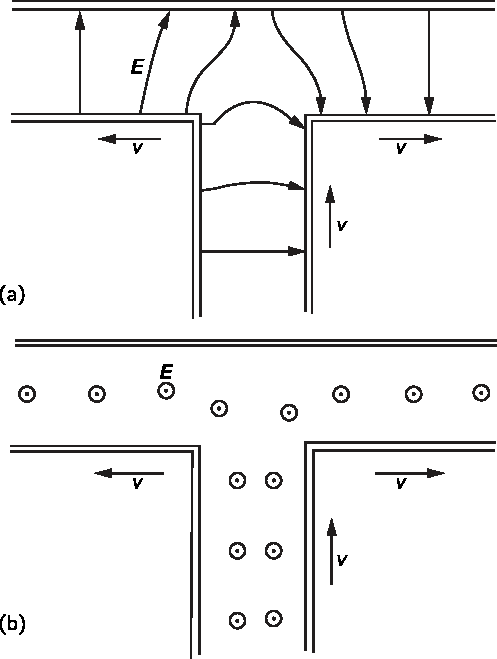
\includegraphics[width=0.7\linewidth]{fyz_fig570.pdf}
      \caption{
               (\cite[s.~707]{Feynman02})}
      \label{fyz:fig570}
    \end{figure}

    \begin{figure}[ht!] %\ref{fyz:fig571}
      \centering
      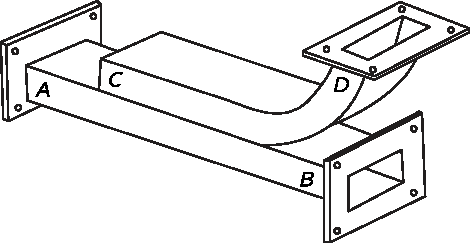
\includegraphics[width=0.7\linewidth]{fyz_fig571.pdf}
      \caption{
               (\cite[s.~707]{Feynman02})}
      \label{fyz:fig571}
    \end{figure}

    \todo[inline]{Kapitola fey2ch24 je nedodělaná, obsahuje pouze obrázky}
%} %tikzset
%---------------------------------------------------------------------------------------------------
